\documentclass{article}

\usepackage[preprint]{neurips_2024}
\usepackage[utf8]{inputenc}
\usepackage[T1]{fontenc}
\usepackage{hyperref}
\usepackage{url}
\usepackage{booktabs}
\usepackage{amsfonts}
\usepackage{amsmath}
\usepackage{nicefrac}
\usepackage{microtype}
\usepackage{xcolor}
\usepackage{graphicx}
\usepackage{float}
\usepackage{tikz}
\usetikzlibrary{arrows.meta,positioning,calc,fit,shapes.geometric,backgrounds}

\definecolor{paperBlue}{HTML}{2F5D9C}
\definecolor{paperCyan}{HTML}{5BB7B5}
\definecolor{paperGreen}{HTML}{66A96B}
\definecolor{paperGold}{HTML}{D8A23A}
\definecolor{paperRed}{HTML}{C75C5C}
\definecolor{paperInk}{HTML}{1F2430}
\definecolor{paperGray}{HTML}{EEF1F5}
\definecolor{paperLilac}{HTML}{B8A8E8}

\title{StreamAvatar: Real-Time Audio-Driven Lip-Synchronized Talking Portrait Generation via Viseme-Guided Motion Latents}

\author{Anonymous Team}

\begin{document}
\maketitle

\begin{abstract}
We propose \textbf{StreamAvatar}, a real-time audio-driven talking portrait system that uses a virtual portrait or avatar image to represent the speaker during live speech. Instead of training a full video generator from scratch, we build a streaming audio-to-mouth-motion module on top of a pretrained portrait renderer. A causal audio encoder with a short look-ahead window predicts viseme states and compact mouth-motion latents; a lightweight flow-matching head models natural coarticulation and uncertainty; and a frozen or lightly adapted renderer converts the predicted motion into lip-synchronized frames. This design targets the practical middle ground between classic real-time lip-sync systems, which are fast but often mechanical, and diffusion-based systems, which are high quality but difficult to deploy interactively. We plan to evaluate on HDTF and LRS3, with MuseTalk and Wav2Lip as deployable baselines and LatentSync as an offline quality reference. Our target is a working demo with 25--30\,fps generation, end-to-end latency under 200\,ms, and visibly stable lip synchronization for a user-controlled virtual identity.
\end{abstract}

%======================================================================
\section{Introduction}
%======================================================================

Audio-driven talking portrait generation aims to synthesize a video of a person or avatar speaking in synchrony with an input audio stream. It is useful for virtual meetings, privacy-preserving telepresence, avatar-based streaming, assistive communication, and low-bandwidth video chat. In our application scenario, a user speaks into a microphone and a virtual portrait represents the user in real time: the identity stays fixed, while the mouth motion follows the speech.

Recent lip-sync methods have made strong progress. Wav2Lip~\cite{wav2lip} introduced a robust SyncNet-based training objective and remains a widely used baseline. MuseTalk~\cite{musetalk} improves real-time video dubbing by performing latent-space inpainting with a VAE and U-Net. LatentSync~\cite{latentsync} pushes synchronization and visual fidelity with audio-conditioned latent diffusion and temporal representation alignment. LivePortrait~\cite{liveportrait} shows that compact implicit keypoints can efficiently drive high-quality portrait animation. DyStream~\cite{dystream} further demonstrates that autoregressive flow-matching models with a small look-ahead window can support ultra-low-latency talking-head generation.

However, practical real-time use still exposes an awkward trade-off. Offline diffusion models can produce attractive details but often require full context and heavy inference. Lightweight real-time systems are fast, yet their mouth motion can be jittery, over-smoothed, or weak under fast speech. We aim to make the core generation problem smaller: rather than generating every pixel causally, \textbf{StreamAvatar predicts compact mouth-motion latents causally and delegates appearance rendering to a pretrained portrait renderer}. In a sense, the renderer handles the expensive makeup; the streaming model only has to decide how the mouth should move.

\textbf{Our key idea} mirrors the structure of the companion StreamLip proposal in the opposite direction. StreamLip uses a text prior to stabilize lip-to-speech synthesis. StreamAvatar uses a viseme prior to stabilize speech-to-lip synthesis. This gives a simple and feasible multimodal learning problem:
\[
    \text{streaming audio} \rightarrow \text{viseme-aware motion latent} \rightarrow \text{lip-synchronized portrait video}.
\]

\begin{figure}[t]
\centering
\resizebox{0.98\textwidth}{!}{%
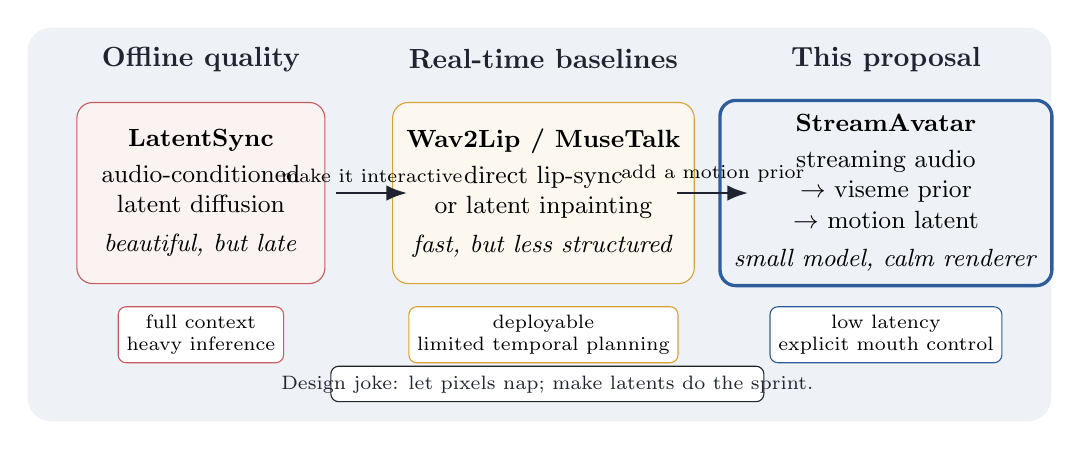
\begin{tikzpicture}[x=1cm,y=1cm,>=Latex,font=\small,
  card/.style={draw=#1,fill=#1!8,rounded corners=2mm,minimum width=3.15cm,minimum height=2.3cm,align=center,inner sep=5pt},
  tag/.style={draw=#1,fill=white,rounded corners=1mm,align=center,inner sep=3pt,font=\scriptsize}
]
  \draw[rounded corners=3mm,fill=paperGray,draw=none] (-0.2,-0.35) rectangle (12.8,4.65);

  \node[font=\bfseries,text=paperInk] at (2.0,4.25) {Offline quality};
  \node[font=\bfseries,text=paperInk] at (6.35,4.25) {Real-time baselines};
  \node[font=\bfseries,text=paperInk] at (10.7,4.25) {This proposal};

  \node[card=paperRed] (offline) at (2.0,2.55)
    {\textbf{LatentSync}\\[2pt]audio-conditioned\\latent diffusion\\[3pt]\textit{beautiful, but late}};
  \node[card=paperGold] (baseline) at (6.35,2.55)
    {\textbf{Wav2Lip / MuseTalk}\\[2pt]direct lip-sync\\or latent inpainting\\[3pt]\textit{fast, but less structured}};
  \node[card=paperBlue,draw=paperBlue,line width=1.2pt] (ours) at (10.7,2.55)
    {\textbf{StreamAvatar}\\[2pt]streaming audio\\$\rightarrow$ viseme prior\\$\rightarrow$ motion latent\\[3pt]\textit{small model, calm renderer}};

  \node[tag=paperRed] at (2.0,0.75) {full context\\heavy inference};
  \node[tag=paperGold] at (6.35,0.75) {deployable\\limited temporal planning};
  \node[tag=paperBlue] at (10.7,0.75) {low latency\\explicit mouth control};

  \draw[->,line width=1.0pt,draw=paperInk] (3.72,2.55) -- node[above,font=\scriptsize] {make it interactive} (4.62,2.55);
  \draw[->,line width=1.0pt,draw=paperInk] (8.05,2.55) -- node[above,font=\scriptsize] {add a motion prior} (8.95,2.55);

  \draw[draw=paperInk,rounded corners=1mm,fill=white] (3.65,-0.1) rectangle (9.15,0.35);
  \node[font=\scriptsize,text=paperInk] at (6.4,0.12) {Design joke: let pixels nap; make latents do the sprint.};
\end{tikzpicture}
}
\caption{Positioning of StreamAvatar. We target low-latency avatar use by generating compact mouth-motion latents instead of directly generating full frames from scratch.}
\label{fig:position}
\end{figure}

%======================================================================
\section{Goal of Achievement}
%======================================================================

Our goal is to demonstrate a working real-time talking portrait system with a fixed virtual identity and streaming speech input. We will focus on a realistic course-project scope: reuse pretrained rendering components, train or fine-tune only the streaming audio-to-motion module, and evaluate both quality and latency.

\paragraph{Target behavior.}
Given a reference portrait image $I$ and a live audio stream $A_{1:t}$, the system outputs a video stream $\hat{X}_{1:t}$ at 25--30\,fps. The mouth should move in synchrony with the spoken content, while the identity, head region, and background remain stable.

\paragraph{Measurable targets.}
We aim for the following outcomes:
\begin{itemize}
    \item \textbf{Latency}: end-to-end latency $\leq$200\,ms, using at most 80--120\,ms of audio look-ahead and a small output buffer.
    \item \textbf{Throughput}: 25--30\,fps on a single modern GPU for a $256{\times}256$ or $512{\times}512$ portrait crop.
    \item \textbf{Lip synchronization}: SyncNet/LSE confidence close to a non-streaming MuseTalk baseline and better than a naively chunked baseline.
    \item \textbf{Temporal stability}: lower mouth-region jitter than a frame-independent baseline.
    \item \textbf{Ablation evidence}: show that the viseme branch and short look-ahead window improve lip-sync quality under streaming constraints.
\end{itemize}

\paragraph{Non-goals.}
We do not claim to train a full high-resolution talking-head generator from scratch. The research contribution is the streaming multimodal control module and the latency-quality trade-off, not a new renderer trained on internet-scale video.

%======================================================================
\section{Methods}
%======================================================================

\subsection{Problem Formulation}

Let $I$ be a reference portrait and $A=\{a_1,\ldots,a_T\}$ be an audio stream. At video frame time $t$, the model may use past audio and a short future context $A_{\leq t+\Delta}$, where $\Delta$ is 80--120\,ms. The system predicts a compact mouth-motion latent $\mathbf{m}_t$ and then renders a frame $\hat{X}_t$:
\begin{equation}
\begin{aligned}
    &p(\hat{X}_{1:T}, \mathbf{m}_{1:T}, \mathbf{v}_{1:T} \mid I, A_{1:T}) \\
    &=
    \prod_{t=1}^{T}
    p(\mathbf{v}_t \mid A_{\leq t+\Delta}, \mathbf{v}_{<t})\,
    p(\mathbf{m}_t \mid A_{\leq t+\Delta}, \mathbf{v}_{\leq t}, \mathbf{m}_{<t})\,
    p(\hat{X}_t \mid I, \mathbf{m}_t).
\end{aligned}
\end{equation}
where $\mathbf{v}_t$ is an auxiliary viseme state. The viseme branch provides a semantic scaffold: it tells the model which family of mouth shape is expected, while the motion latent branch decides the continuous intensity, timing, and transition.

\subsection{Architecture}

\begin{figure}[t]
\centering
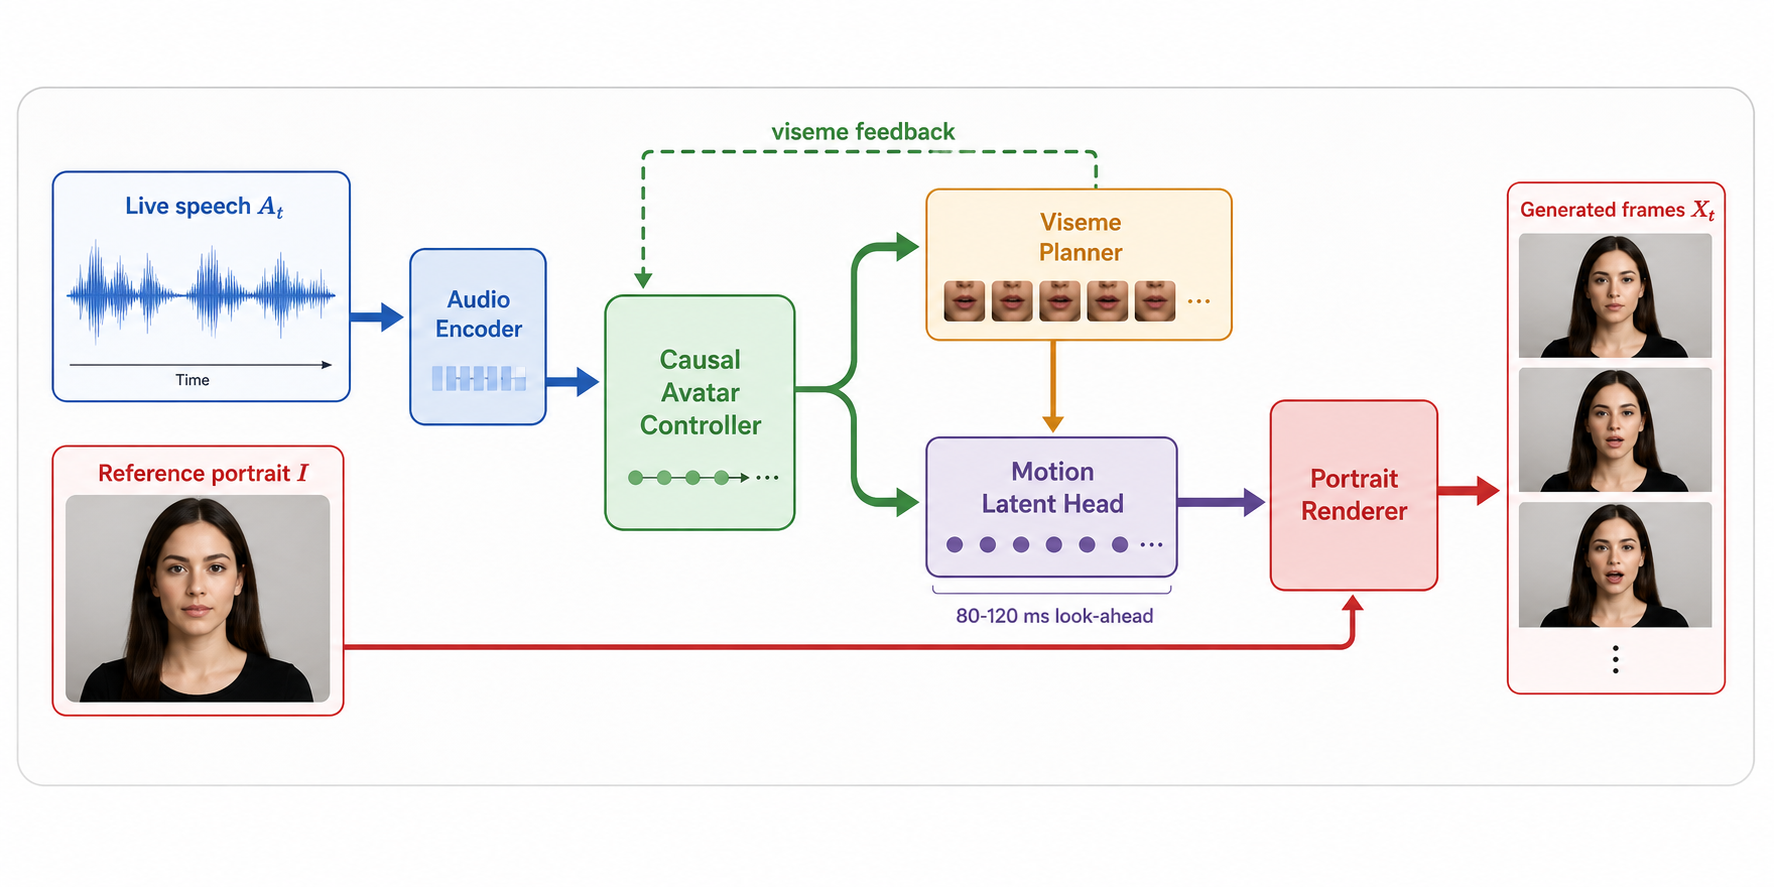
\includegraphics[width=\textwidth]{fig_streamavatar_arch_gpt.png}
\caption{StreamAvatar architecture. The audio stream is encoded causally, a viseme branch supplies a semantic mouth-shape prior, and a motion latent head drives a pretrained portrait renderer.}
\label{fig:arch}
\end{figure}

\paragraph{Audio front-end.}
We use a frozen audio encoder such as Whisper-tiny~\cite{whisper}, wav2vec~2.0~\cite{wav2vec2}, or HuBERT~\cite{hubert}. The encoder is run on sliding chunks, producing frame-aligned audio features. Freezing the front-end reduces training cost and makes the project feasible.

\paragraph{Streaming adapter.}
A small causal Conformer or Transformer consumes audio features and previous mouth states. It uses limited look-ahead attention inside a local window and causal attention across windows. This follows the practical lesson from streaming generation systems: a tiny amount of future context often buys a large quality gain without destroying interactivity.

\paragraph{Viseme branch.}
A linear head predicts a viseme token $\mathbf{v}_t$ at each frame. Viseme labels can be obtained from forced-aligned transcripts when available, or from ASR transcripts followed by a grapheme-to-phoneme and phoneme-to-viseme mapping. During training, the viseme branch is supervised by cross-entropy or CTC:
\begin{equation}
    \mathcal{L}_{\text{vis}} = - \sum_t \log p(\mathbf{v}_t \mid \mathbf{h}_t).
\end{equation}
During inference, the continuous hidden state and the predicted viseme distribution are both passed to the motion head. This keeps uncertainty information instead of collapsing everything to a hard token.

\paragraph{Motion latent flow-matching head.}
The output target $\mathbf{m}_t$ can be one of two implementation-friendly representations:
\begin{itemize}
    \item \textbf{MuseTalk-compatible latent}: mouth-region VAE latent or U-Net conditioning residual used for latent inpainting.
    \item \textbf{LivePortrait-compatible motion}: implicit keypoint offsets or retargeting coefficients used by a fast portrait renderer.
\end{itemize}
We model $\mathbf{m}_t$ with a lightweight flow-matching head. Given noise $\mathbf{x}_0 \sim \mathcal{N}(0,I)$ and target latent $\mathbf{x}_1=\mathbf{m}_t$, the model learns the vector field
\begin{equation}
    \mathcal{L}_{\text{FM}}
    =
    \mathbb{E}_{t,\mathbf{x}_0,\mathbf{x}_1}
    \left\|
    v_\theta(\mathbf{x}_\tau,\tau \mid \mathbf{h}_t, \mathbf{v}_t, \mathbf{m}_{t-1})
    -
    (\mathbf{x}_1-\mathbf{x}_0)
    \right\|^2,
    \quad
    \mathbf{x}_\tau=(1-\tau)\mathbf{x}_0+\tau\mathbf{x}_1.
\end{equation}
At inference, we use a small number of Euler steps. If the flow head is too expensive for the course timeline, we keep the same architecture and replace it with deterministic latent regression as an ablation and fallback.

\paragraph{Renderer.}
The renderer is pretrained and reused. Our first engineering baseline will be MuseTalk because it already provides real-time lip-sync inference and pretrained weights. A LivePortrait-style renderer is attractive for a later stage because its motion representation is compact and controllable. In both cases, the renderer is frozen initially, and only small adapters are trained if necessary.

\subsection{Training Strategy}

We train in three phases:
\begin{enumerate}
    \item \textbf{Baseline reproduction.} Run Wav2Lip and MuseTalk on the target evaluation clips and record latency, FPS, and synchronization metrics. This gives a non-negotiable sanity check before adding new modules.
    \item \textbf{Streaming adapter pretraining.} Train the audio encoder adapter and viseme head on paired audio-video clips from HDTF and LRS3. The target mouth motion is extracted from the pretrained renderer's latent interface or from tracked landmarks.
    \item \textbf{End-to-end adapter tuning.} Freeze the main renderer and tune only the streaming adapter, viseme head, and motion latent head with reconstruction, synchronization, and temporal losses.
\end{enumerate}

The full loss is
\begin{equation}
    \mathcal{L}
    =
    \mathcal{L}_{\text{FM}}
    + \lambda_{\text{vis}}\mathcal{L}_{\text{vis}}
    + \lambda_{\text{sync}}\mathcal{L}_{\text{sync}}
    + \lambda_{\text{rec}}\mathcal{L}_{\text{rec}}
    + \lambda_{\text{smooth}}\mathcal{L}_{\text{smooth}}.
\end{equation}
Here $\mathcal{L}_{\text{sync}}$ is a SyncNet-based lip-audio loss~\cite{syncnet,wav2lip}, $\mathcal{L}_{\text{rec}}$ is a mouth-region latent or pixel reconstruction loss, and $\mathcal{L}_{\text{smooth}}$ penalizes high-frequency mouth jitter. We will also use scheduled condition corruption: occasionally masking the viseme distribution or previous-motion input so the model does not become brittle when streaming predictions are imperfect.

\subsection{Streaming Inference}

\begin{figure}[H]
\centering
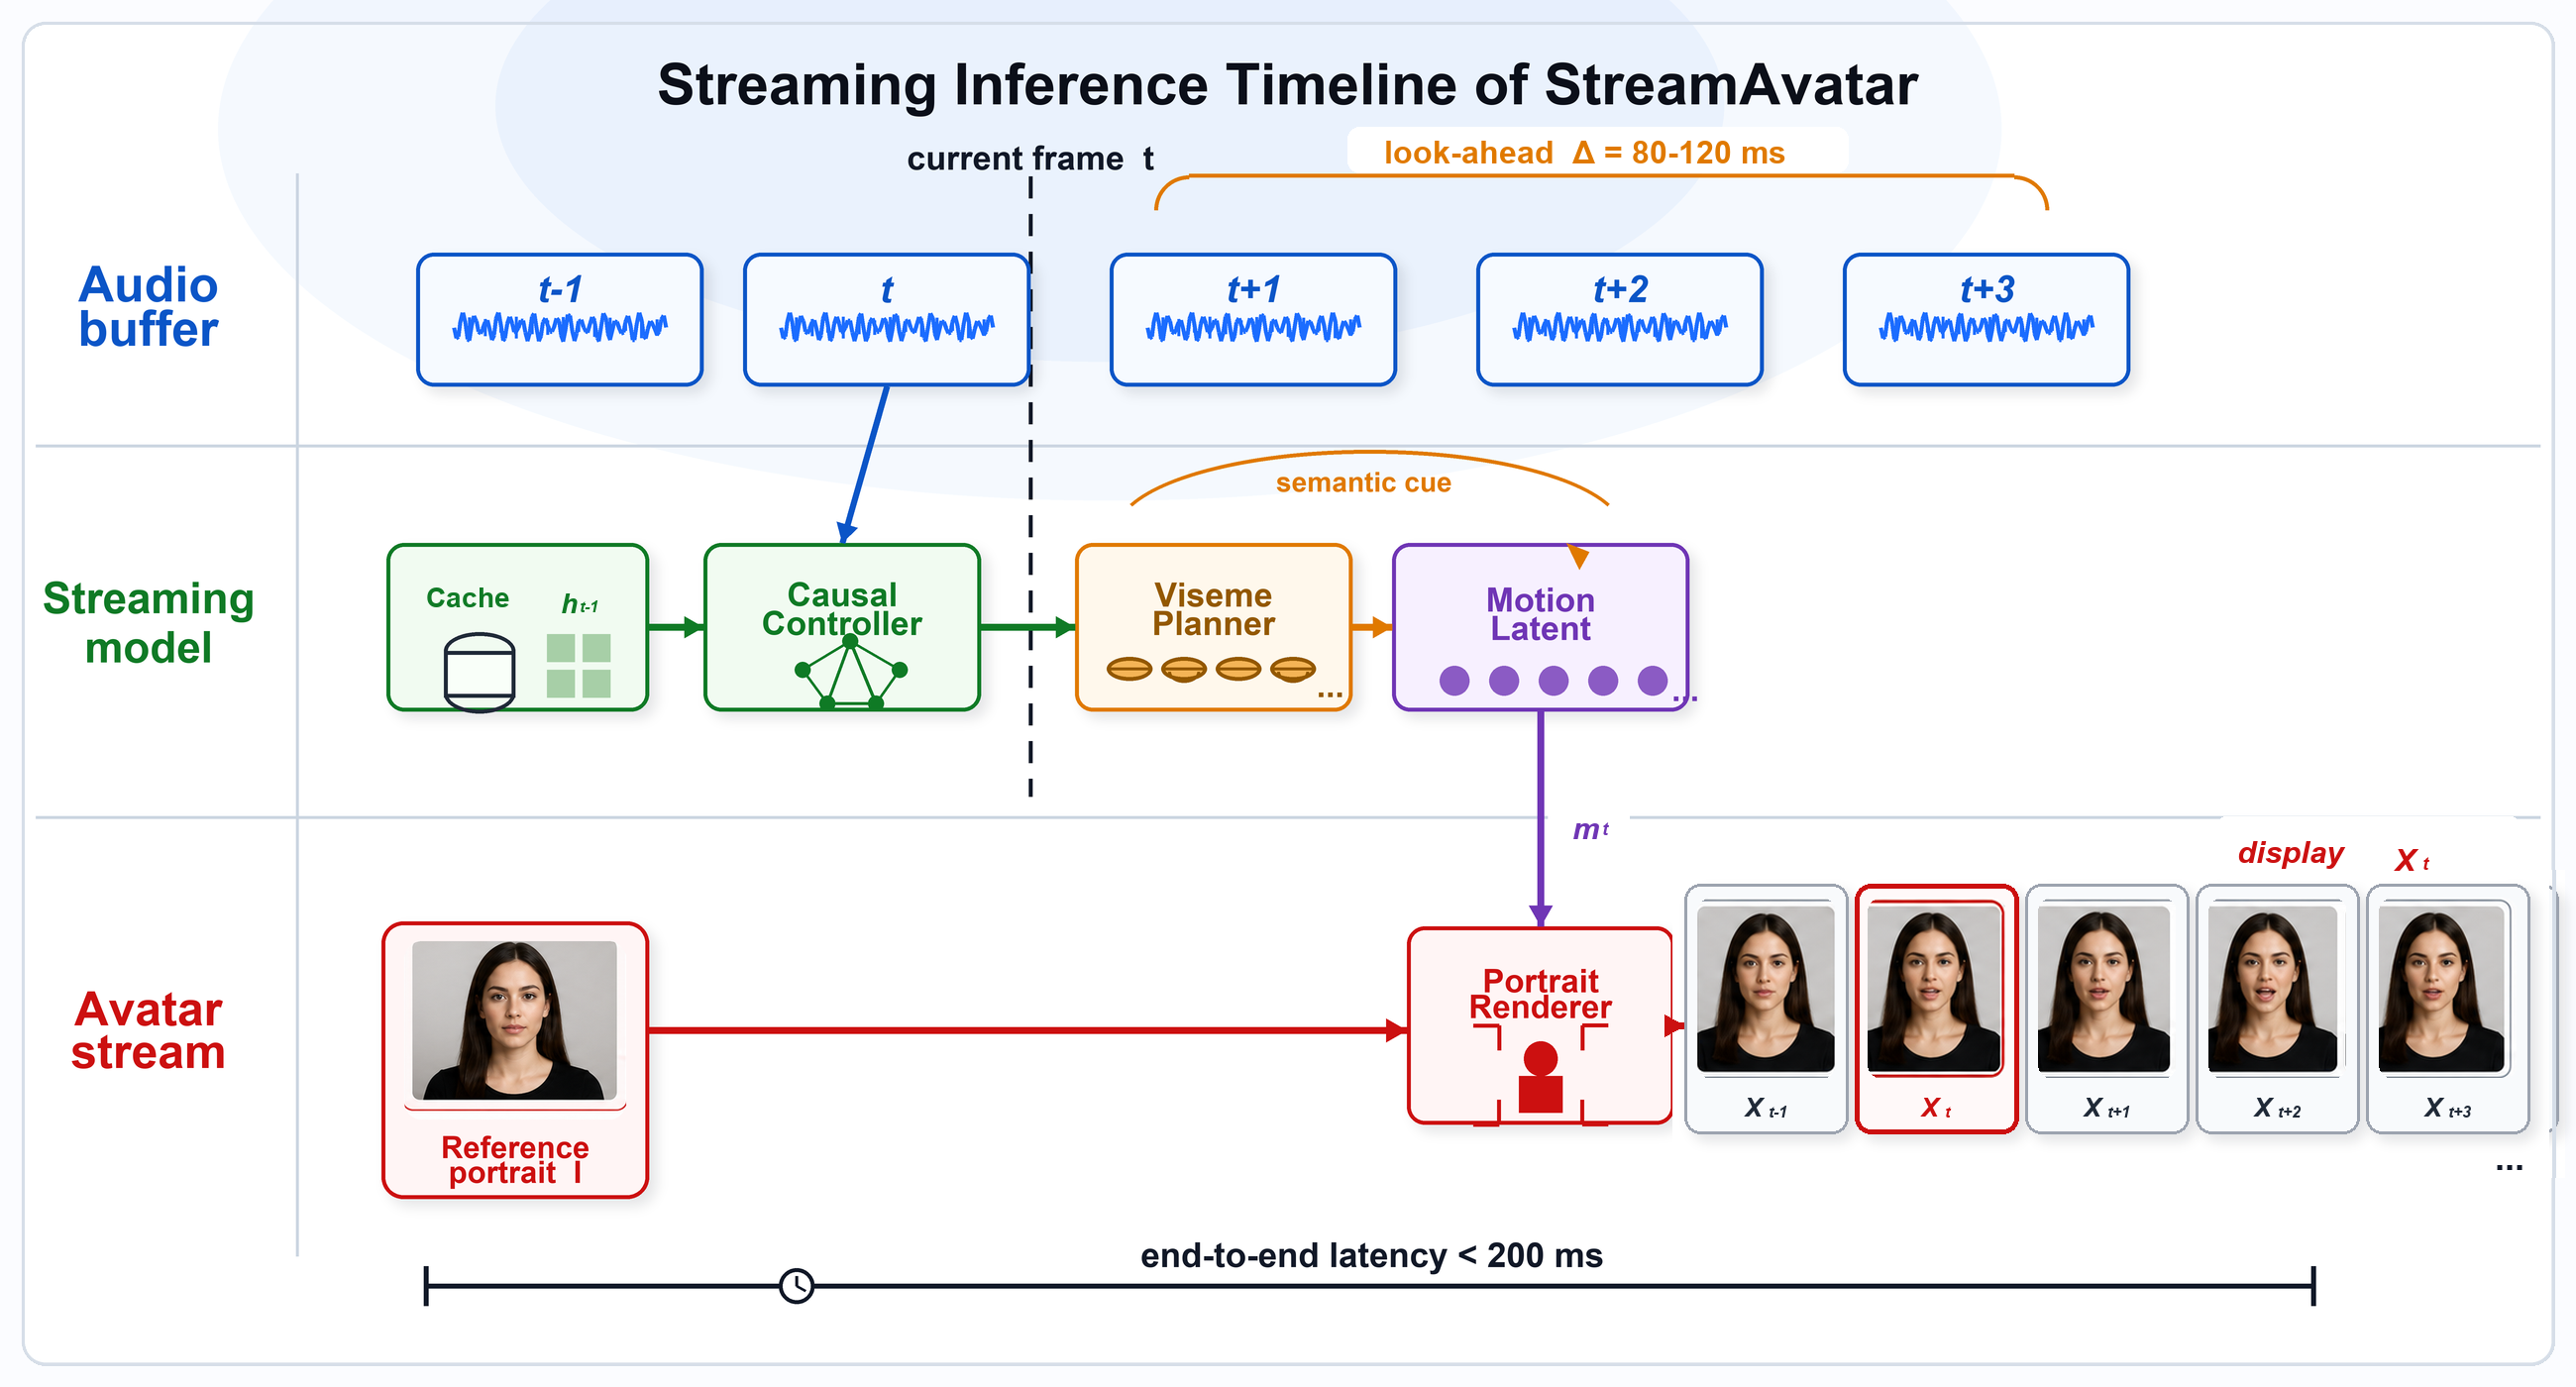
\includegraphics[width=\textwidth]{fig_streamavatar_timeline_gpt.png}
\iffalse
\resizebox{\textwidth}{!}{%
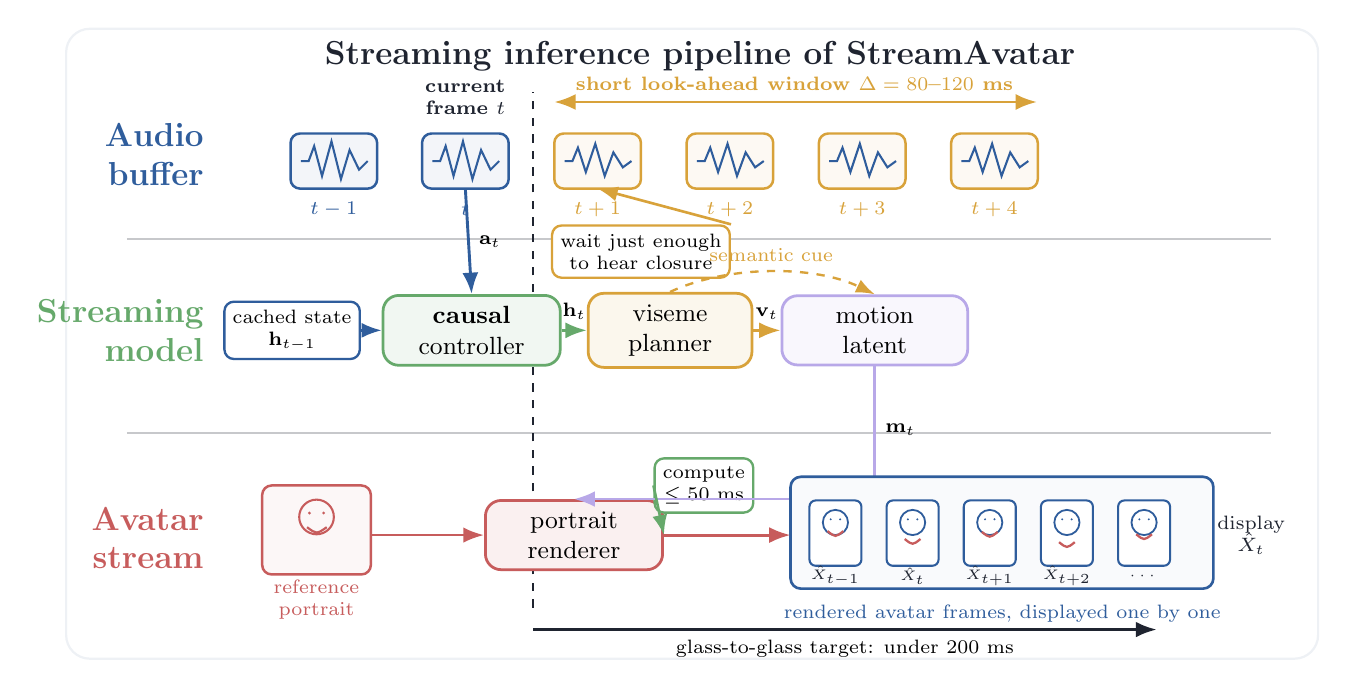
\begin{tikzpicture}[x=1cm,y=1cm,>=Latex,font=\small,
  lane/.style={font=\bfseries\large,text=#1,align=right,anchor=east},
  op/.style={draw=#1,fill=#1!9,rounded corners=2mm,line width=1.0pt,minimum width=2.10cm,minimum height=0.82cm,align=center,inner sep=4pt},
  callout/.style={draw=#1,fill=white,rounded corners=1.2mm,line width=0.85pt,align=center,inner sep=3pt,font=\scriptsize},
  chunk/.style={draw=#1,fill=#1!6,rounded corners=1.2mm,line width=0.9pt}
]
  \draw[rounded corners=3mm,fill=white,draw=paperGray,line width=0.8pt]
    (-0.15,-0.15) rectangle (15.75,7.85);
  \node[font=\bfseries\large,text=paperInk] at (7.90,7.50)
    {Streaming inference pipeline of StreamAvatar};
  \draw[draw=paperInk!25,line width=0.8pt] (0.62,5.18) -- (15.15,5.18);
  \draw[draw=paperInk!25,line width=0.8pt] (0.62,2.72) -- (15.15,2.72);

  \node[lane=paperBlue] at (1.72,6.25) {Audio\\buffer};
  \node[lane=paperGreen] at (1.72,4.02) {Streaming\\model};
  \node[lane=paperRed] at (1.72,1.38) {Avatar\\stream};

  \foreach \x/\lab in {3.25/$t-1$,4.92/$t$} {
    \draw[chunk=paperBlue] (\x-0.55,5.82) rectangle (\x+0.55,6.52);
    \draw[draw=paperBlue,line width=0.75pt]
      (\x-0.42,6.17) -- (\x-0.32,6.17) -- (\x-0.25,6.36) --
      (\x-0.15,5.98) -- (\x-0.03,6.42) -- (\x+0.09,5.94) --
      (\x+0.20,6.31) -- (\x+0.32,6.06) -- (\x+0.43,6.17);
    \node[font=\scriptsize,text=paperBlue] at (\x,5.55) {\lab};
  }
  \foreach \x/\lab in {6.60/$t+1$,8.28/$t+2$,9.96/$t+3$,11.64/$t+4$} {
    \draw[chunk=paperGold] (\x-0.55,5.82) rectangle (\x+0.55,6.52);
    \draw[draw=paperBlue,line width=0.75pt]
      (\x-0.42,6.17) -- (\x-0.32,6.17) -- (\x-0.25,6.34) --
      (\x-0.15,6.03) -- (\x-0.03,6.39) -- (\x+0.09,5.98) --
      (\x+0.20,6.28) -- (\x+0.32,6.09) -- (\x+0.43,6.17);
    \node[font=\scriptsize,text=paperGold] at (\x,5.55) {\lab};
  }

  \draw[draw=paperInk,dashed,line width=0.9pt] (5.78,0.50) -- (5.78,7.05);
  \node[font=\bfseries\scriptsize,text=paperInk,align=center] at (4.92,6.98)
    {current\\frame $t$};
  \draw[<->,draw=paperGold,line width=1.05pt] (6.05,6.92) -- (12.18,6.92);
  \node[font=\bfseries\scriptsize,text=paperGold] at (9.10,7.15)
    {short look-ahead window $\Delta=80$--$120$ ms};

  \node[callout=paperBlue] (cache) at (2.72,4.02)
    {cached state\\$\mathbf{h}_{t-1}$};
  \node[op=paperGreen,minimum width=2.25cm] (ctrl) at (5.00,4.02)
    {\textbf{causal}\\controller};
  \node[op=paperGold,minimum width=2.08cm] (vis) at (7.52,4.02)
    {viseme\\planner};
  \node[op=paperLilac,minimum width=2.36cm] (motion) at (10.12,4.02)
    {motion\\latent};
  \node[callout=paperGold] (wait) at (7.15,5.02)
    {wait just enough\\to hear closure};

  \draw[->,line width=1.05pt,draw=paperBlue] (4.92,5.82) -- node[right,font=\scriptsize] {$\mathbf{a}_t$} (ctrl.north);
  \draw[->,line width=0.95pt,draw=paperBlue] (cache.east) -- (ctrl.west);
  \draw[->,line width=1.05pt,draw=paperGreen] (ctrl.east) -- node[above,font=\scriptsize] {$\mathbf{h}_t$} (vis.west);
  \draw[->,line width=1.05pt,draw=paperGold] (vis.east) -- node[above,font=\scriptsize] {$\mathbf{v}_t$} (motion.west);
  \draw[->,line width=0.95pt,draw=paperGold] (wait.north east) -- (6.60,5.82);
  \draw[->,dashed,line width=0.85pt,draw=paperGold]
    (vis.north) .. controls (8.25,4.85) and (9.35,4.85) .. node[above,font=\scriptsize,text=paperGold] {semantic cue} (motion.north);

  \draw[rounded corners=1.2mm,draw=paperRed,fill=paperRed!5,line width=0.9pt]
    (2.34,0.92) rectangle (3.72,2.05);
  \draw[draw=paperRed,line width=0.75pt] (3.03,1.65) circle (0.22);
  \fill[paperRed] (2.94,1.70) circle (0.02);
  \fill[paperRed] (3.12,1.70) circle (0.02);
  \draw[draw=paperRed,line width=0.8pt] (2.91,1.52) .. controls (3.03,1.43) .. (3.16,1.52);
  \node[font=\scriptsize,text=paperRed,align=center] at (3.03,0.60)
    {reference\\portrait};

  \node[op=paperRed,minimum width=2.25cm] (renderer) at (6.30,1.42)
    {portrait\\renderer};
  \node[callout=paperGreen] (compute) at (7.95,2.05) {compute\\$\leq 50$ ms};
  \draw[->,line width=1.00pt,draw=paperRed] (3.72,1.42) -- (renderer.west);
  \draw[->,line width=1.00pt,draw=paperLilac] (motion.south) |- node[pos=.24,right,font=\scriptsize] {$\mathbf{m}_t$} (renderer.north);
  \draw[->,line width=0.95pt,draw=paperGreen] (compute.west) -- (renderer.east);

  \draw[rounded corners=1.3mm,draw=paperBlue,fill=paperBlue!3,line width=0.95pt]
    (9.05,0.74) rectangle (14.42,2.16);
  \foreach \x/\mouth/\lab in {9.62/0.02/$\hat{X}_{t-1}$,10.60/0.12/$\hat{X}_t$,11.58/0.03/$\hat{X}_{t+1}$,12.56/0.16/$\hat{X}_{t+2}$,13.54/0.06/$\cdots$} {
    \draw[rounded corners=0.8mm,draw=paperBlue,fill=white,line width=0.75pt]
      (\x-0.33,1.03) rectangle (\x+0.33,1.86);
    \draw[draw=paperBlue,line width=0.65pt] (\x,1.58) circle (0.16);
    \fill[paperBlue] (\x-0.06,1.62) circle (0.014);
    \fill[paperBlue] (\x+0.06,1.62) circle (0.014);
    \draw[draw=paperRed,line width=0.82pt]
      (\x-0.10,1.49-\mouth) .. controls (\x,1.41-\mouth) .. (\x+0.10,1.49-\mouth);
    \node[font=\tiny,text=paperInk] at (\x,0.90) {\lab};
  }
  \node[font=\scriptsize,text=paperBlue,align=center] at (11.74,0.42)
    {rendered avatar frames, displayed one by one};
  \draw[->,line width=1.05pt,draw=paperRed] (renderer.east) -- (9.05,1.42);
  \node[font=\scriptsize,text=paperInk,align=center] at (14.90,1.42)
    {display\\$\hat{X}_t$};

  \draw[->,line width=1.0pt,draw=paperInk] (5.78,0.22) -- node[below,font=\scriptsize]
    {glass-to-glass target: under 200 ms} (13.70,0.22);
\end{tikzpicture}
}
\fi
\caption{Streaming schedule. A small future audio window helps the model anticipate mouth closure and vowel transitions, while the portrait renderer turns each predicted mouth latent into an avatar frame under the interactive latency budget.}
\label{fig:timeline}
\end{figure}

At runtime, the system loops over video-frame timestamps:
\begin{enumerate}
    \item Collect the audio window ending at $t+\Delta$.
    \item Encode audio features and update the causal adapter cache.
    \item Predict the viseme distribution and mouth-motion latent.
    \item Render the current frame with the pretrained portrait renderer.
    \item Apply lightweight temporal smoothing and display the frame.
\end{enumerate}
We will implement the streaming wrapper so that offline audio files and live microphone input use the same buffering code. This makes it easy to debug deterministically on saved audio and then switch to a live demo.

%======================================================================
\section{Experiments}
%======================================================================

\subsection{Datasets}

We will primarily use HDTF~\cite{hdtf} for talking-head clips and LRS3~\cite{lrs3} for speech-rich audio-video examples. If compute is limited, we will train on a curated subset with clean frontal faces and evaluate on held-out speakers. Preprocessing follows common talking-head pipelines: face detection, landmark alignment, mouth crop extraction, and audio-video synchronization checks.

\subsection{Baselines}

\begin{itemize}
    \item \textbf{Wav2Lip}: classic robust lip-sync baseline.
    \item \textbf{MuseTalk}: strongest practical real-time baseline and engineering starting point.
    \item \textbf{Chunked MuseTalk}: MuseTalk forced into small audio chunks; this tests whether naive chunking is enough.
    \item \textbf{LatentSync}: offline high-quality reference, not expected to satisfy our latency budget.
    \item \textbf{Ours w/o viseme branch}: ablation for the semantic mouth-shape prior.
    \item \textbf{Ours w/o look-ahead}: ablation for short future context.
\end{itemize}

\subsection{Metrics}

We evaluate:
\begin{itemize}
    \item \textbf{Lip synchronization}: LSE-D and LSE-C from SyncNet.
    \item \textbf{Visual quality}: FID/FVD or LPIPS on the mouth region, plus qualitative examples.
    \item \textbf{Identity preservation}: ArcFace cosine similarity between generated and reference frames.
    \item \textbf{Temporal stability}: mouth landmark jitter and frame-to-frame latent variation.
    \item \textbf{System performance}: FPS, per-frame compute time, look-ahead size, and end-to-end latency.
    \item \textbf{User preference}: small human study comparing our streaming output with Wav2Lip and MuseTalk under the same avatar image.
\end{itemize}

%======================================================================
\section{Feasibility and Risks}
%======================================================================

\paragraph{Why this is feasible.}
The project does not require collecting a new dataset or training a full generator. Pretrained systems already provide the heavy visual prior. Our trainable part is small: a causal temporal adapter, a viseme head, and a motion latent head. A meaningful demo can be produced even if training is limited, because MuseTalk or Wav2Lip can serve as an initial renderer/baseline.

\paragraph{Main risks.}
The first risk is that the renderer's internal latent interface may not be clean enough for direct motion-latent supervision. If so, we will supervise mouth landmarks or VAE latents instead. The second risk is that flow matching may be too slow under the latency budget. If this happens, deterministic regression becomes the deployable model, and flow matching remains an offline ablation. The third risk is dataset preprocessing time. We mitigate it by starting with pretrained inference and a small clean subset rather than full-scale training.

\paragraph{Ethical use.}
Talking portrait systems can be misused for impersonation. Our demo will use consented images or synthetic/virtual portraits, add an optional visual watermark, and frame the application as avatar-based representation rather than identity deception.

%======================================================================
\section{Timeline}
%======================================================================

\begin{table}[h]
\centering
\small
\begin{tabular}{@{}lll@{}}
\toprule
\textbf{Period} & \textbf{Milestone} & \textbf{Deliverable} \\
\midrule
Week 1 & Baseline reproduction & Wav2Lip/MuseTalk running; latency and SyncNet metrics \\
Week 2 & Streaming wrapper & Chunked audio buffer, causal cache, live/offline demo path \\
Week 3 & Viseme-guided adapter & Trainable adapter, viseme branch, motion latent loss \\
Week 4 & Evaluation and writing & Ablations, final report, demo video, poster figures \\
\bottomrule
\end{tabular}
\end{table}

%======================================================================
\section{Workload Distribution}
%======================================================================

\begin{table}[h]
\centering
\small
\begin{tabular}{@{}ll@{}}
\toprule
\textbf{Member} & \textbf{Responsibilities} \\
\midrule
Member 1 & Renderer integration; MuseTalk/Wav2Lip baselines; demo pipeline \\
Member 2 & Data preprocessing; streaming audio buffer; evaluation metrics \\
Member 3 & Model architecture; viseme branch; motion latent and flow-matching head \\
\midrule
All & Literature review; qualitative analysis; report writing; presentation \\
\bottomrule
\end{tabular}
\end{table}

\bibliographystyle{unsrt}
\bibliography{ref}

\end{document}
